\documentclass[aspectratio=169,11pt]{beamer}

% Theme
\usetheme{Madrid}
\usecolortheme{whale}
\setbeamertemplate{navigation symbols}{}
\setbeamertemplate{footline}[frame number]

% Packages
\usepackage{graphicx}
\usepackage{booktabs}
\usepackage{amsmath}
\usepackage{tikz}
\usetikzlibrary{shapes,arrows,positioning,calc}
\usepackage{xcolor}
\usepackage{listings}

% Colors
\definecolor{celegans}{RGB}{76,153,0}
\definecolor{contact}{RGB}{204,102,0}
\definecolor{lineage}{RGB}{51,102,204}

% Title
\title[NemaContext]{NemaContext: Generative Modeling of\\Complete Embryo Development}
\subtitle{Progress Report: Data Integration \& Contact Graph Prediction}
\author{Progress Report}
\date{\today}

\begin{document}

% ============================================================
% Title Slide
% ============================================================
\begin{frame}
\titlepage
\end{frame}

% ============================================================
% Outline
% ============================================================
\begin{frame}{Outline}
\tableofcontents
\end{frame}

% ============================================================
\section{Project Vision}
% ============================================================

\begin{frame}{The Grand Challenge: Digital Embryogenesis}
\begin{columns}
\column{0.55\textwidth}
\textbf{Goal}: Generate complete embryo states from a single zygote

\vspace{0.5em}
\begin{block}{Input $\rightarrow$ Output}
\begin{itemize}
    \item \textbf{Input}: Zygote state at $t=0$ (1 cell)
    \item \textbf{Output}: Complete embryo at any time $t$
    \begin{itemize}
        \item Every cell's transcriptome
        \item Every cell's 3D position
        \item \textcolor{contact}{Cell-cell neighbor relationships}
        \item Lineage tree structure
    \end{itemize}
\end{itemize}
\end{block}

\column{0.42\textwidth}
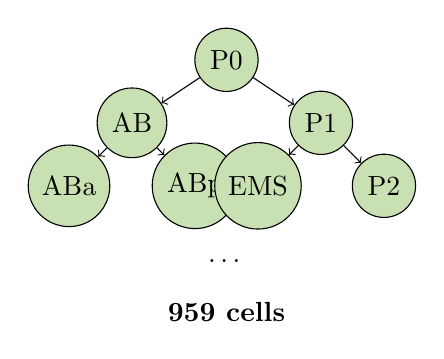
\begin{tikzpicture}[scale=0.8]
    % Tree structure
    \node[circle,draw,fill=celegans!30] (p0) at (0,4) {P0};
    \node[circle,draw,fill=celegans!30] (ab) at (-1.5,3) {AB};
    \node[circle,draw,fill=celegans!30] (p1) at (1.5,3) {P1};
    \node[circle,draw,fill=celegans!30] (aba) at (-2.5,2) {ABa};
    \node[circle,draw,fill=celegans!30] (abp) at (-0.5,2) {ABp};
    \node[circle,draw,fill=celegans!30] (ems) at (0.5,2) {EMS};
    \node[circle,draw,fill=celegans!30] (p2) at (2.5,2) {P2};
    
    \draw[->] (p0) -- (ab);
    \draw[->] (p0) -- (p1);
    \draw[->] (ab) -- (aba);
    \draw[->] (ab) -- (abp);
    \draw[->] (p1) -- (ems);
    \draw[->] (p1) -- (p2);
    
    \node at (0,0.8) {\dots};
    \node at (0,0) {\textbf{959 cells}};
\end{tikzpicture}
\end{columns}
\end{frame}

\begin{frame}{Why \textit{C. elegans}?}
\begin{columns}
\column{0.48\textwidth}
\begin{block}{Unique Properties}
\begin{itemize}
    \item \textbf{Invariant lineage}: 100\% deterministic cell divisions
    \item \textbf{Complete spatial tracking}: WormGUIDES 4D atlas
    \item \textbf{Lineage-resolved transcriptomics}: Large et al. 2025
    \item \textbf{Small cell count}: 959 cells (tractable)
    \item \textbf{Extensive ground truth}: Decades of research
\end{itemize}
\end{block}

\column{0.48\textwidth}
\begin{block}{Cell as Token Paradigm}
\begin{itemize}
    \item Each cell $\rightarrow$ A token
    \item Development $\rightarrow$ Tree generation
    \item Cell division $\rightarrow$ Token splits into two
    \item Zygote $\rightarrow$ Adult: 1 $\rightarrow$ 959 tokens
\end{itemize}
\end{block}
\end{columns}

\vspace{1em}
\centering
\textit{C. elegans is the \textbf{only} multicellular organism where complete generative modeling is feasible.}
\end{frame}

% ============================================================
\section{Data Integration Progress}
% ============================================================

\begin{frame}{Trimodal Data Integration}
\begin{center}
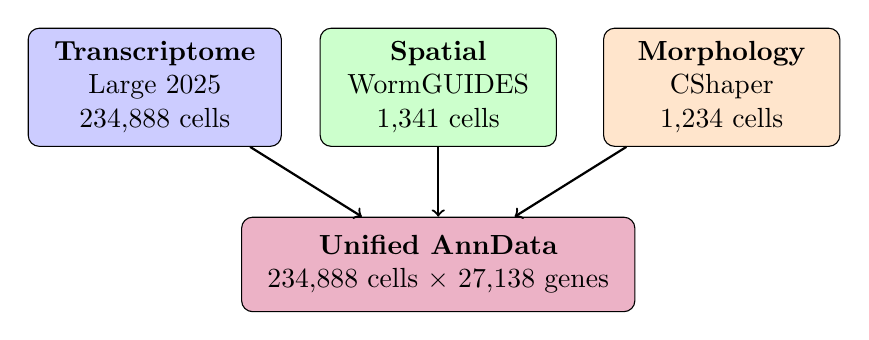
\begin{tikzpicture}[scale=0.9]
    % Three modalities
    \node[draw,rounded corners,fill=blue!20,minimum width=3cm,minimum height=1.5cm] (expr) at (-4,0) {
        \begin{tabular}{c}
        \textbf{Transcriptome}\\
        Large 2025\\
        234,888 cells
        \end{tabular}
    };
    
    \node[draw,rounded corners,fill=green!20,minimum width=3cm,minimum height=1.5cm] (space) at (0,0) {
        \begin{tabular}{c}
        \textbf{Spatial}\\
        WormGUIDES\\
        1,341 cells
        \end{tabular}
    };
    
    \node[draw,rounded corners,fill=orange!20,minimum width=3cm,minimum height=1.5cm] (morph) at (4,0) {
        \begin{tabular}{c}
        \textbf{Morphology}\\
        CShaper\\
        1,234 cells
        \end{tabular}
    };
    
    % Center
    \node[draw,rounded corners,fill=purple!30,minimum width=3.5cm,minimum height=1.2cm] (anndata) at (0,-2.5) {
        \begin{tabular}{c}
        \textbf{Unified AnnData}\\
        234,888 cells $\times$ 27,138 genes
        \end{tabular}
    };
    
    % Arrows
    \draw[->,thick] (expr) -- (anndata);
    \draw[->,thick] (space) -- (anndata);
    \draw[->,thick] (morph) -- (anndata);
\end{tikzpicture}
\end{center}
\end{frame}

\begin{frame}{CShaper Integration: Key Achievement}
\begin{block}{What is CShaper?}
4D morphological atlas of \textit{C. elegans} embryo (Cao et al. 2020)
\begin{itemize}
    \item \textbf{Cell-cell contact matrices}: Physical neighbor relationships
    \item \textbf{Cell morphology}: Volume, surface area, sphericity
    \item \textbf{Standardized coordinates}: Averaged across 46 embryos
\end{itemize}
\end{block}

\vspace{0.5em}

\begin{columns}
\column{0.48\textwidth}
\begin{block}{Integration Results}
\begin{tabular}{lr}
\toprule
Metric & Value \\
\midrule
Cells with morphology & 94,005 (40\%) \\
Direct matches & 25,264 \\
Ancestor-mapped & 1,390 \\
Contact edges & 1,854,781 \\
\bottomrule
\end{tabular}
\end{block}

\column{0.48\textwidth}
\begin{block}{Matching Strategies}
\begin{enumerate}
    \item \textbf{Direct}: Cell exists in CShaper
    \item \textbf{Fuzzy}: Handle `x' and `/' in lineage
    \item \textbf{Ancestor}: Map to closest ancestor
    \item \textbf{Expression}: Validate with gene expression
\end{enumerate}
\end{block}
\end{columns}
\end{frame}

% ============================================================
\section{The Contact Graph Problem}
% ============================================================

\begin{frame}{The Temporal Coverage Gap}
\begin{center}
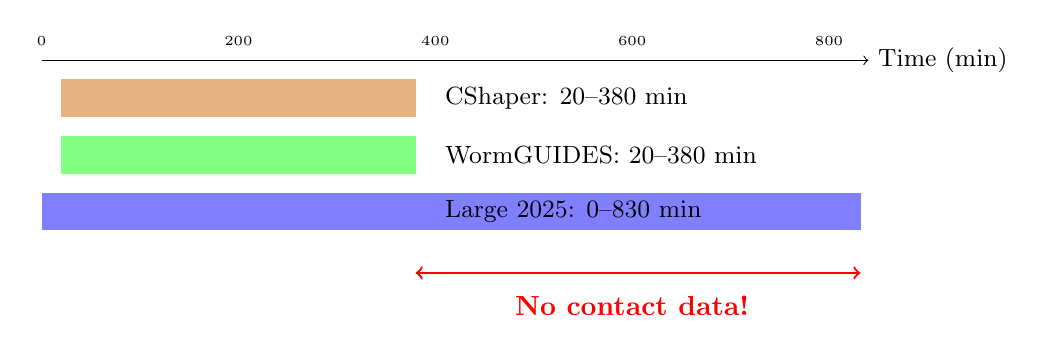
\begin{tikzpicture}[xscale=1,yscale=0.6]
    % Timeline (scaled to 0-10 representing 0-800 min)
    \draw[->] (0,0) -- (10.5,0) node[right] {\small Time (min)};
    
    % CShaper coverage (20-380 min -> 0.25-4.75)
    \fill[contact!50] (0.25,-1.2) rectangle (4.75,-0.4);
    \node[right] at (5,-0.8) {\small CShaper: 20--380 min};
    
    % WormGUIDES coverage
    \fill[green!50] (0.25,-2.4) rectangle (4.75,-1.6);
    \node[right] at (5,-2.0) {\small WormGUIDES: 20--380 min};
    
    % Large2025 coverage (0-830 min -> 0-10.4)
    \fill[blue!50] (0,-3.6) rectangle (10.4,-2.8);
    \node[right] at (5,-3.2) {\small Large 2025: 0--830 min};
    
    % Axis labels
    \node[above] at (0,0.1) {\tiny 0};
    \node[above] at (2.5,0.1) {\tiny 200};
    \node[above] at (5,0.1) {\tiny 400};
    \node[above] at (7.5,0.1) {\tiny 600};
    \node[above] at (10,0.1) {\tiny 800};
    
    % Gap annotation
    \draw[<->,red,thick] (4.75,-4.5) -- (10.4,-4.5);
    \node[red] at (7.5,-5.2) {\textbf{No contact data!}};
\end{tikzpicture}
\end{center}

\vspace{0.5em}
\textbf{Problem}: We have transcriptomes for late-stage cells (380--830 min), but \textbf{no spatial/contact information}!

\vspace{0.5em}
\textbf{Question}: Can we \textcolor{contact}{\textbf{predict}} contact relationships for late-stage cells?
\end{frame}

\begin{frame}{Initial Approach: Ancestor Mapping (Incorrect)}
\begin{columns}
\column{0.48\textwidth}
\textbf{Na\"ive Approach}:
\begin{itemize}
    \item Map late-stage cells to their early ancestors
    \item If ancestors A and B contacted $\rightarrow$ all descendants of A contact all descendants of B
    \item Result: 50 million edges!
\end{itemize}

\vspace{0.5em}
\textcolor{red}{\textbf{Biologically incorrect!}}
\begin{itemize}
    \item Ancestor contact $\neq$ descendant contact
    \item Cells migrate, tissues reorganize
    \item Late-stage spatial arrangement differs from early
\end{itemize}

\column{0.48\textwidth}
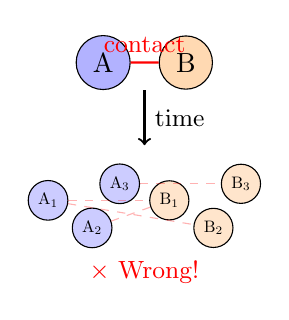
\begin{tikzpicture}[scale=0.7]
    % Early stage
    \node[circle,draw,fill=blue!30] (a) at (0,3) {A};
    \node[circle,draw,fill=orange!30] (b) at (1.5,3) {B};
    \draw[thick,red] (a) -- (b) node[midway,above] {\small contact};
    
    % Arrow
    \draw[->,thick] (0.75,2.5) -- (0.75,1.5) node[midway,right] {\small time};
    
    % Late stage - descendants
    \node[circle,draw,fill=blue!20,scale=0.6] (a1) at (-1,0.5) {A$_1$};
    \node[circle,draw,fill=blue!20,scale=0.6] (a2) at (-0.2,0) {A$_2$};
    \node[circle,draw,fill=blue!20,scale=0.6] (a3) at (0.3,0.8) {A$_3$};
    \node[circle,draw,fill=orange!20,scale=0.6] (b1) at (1.2,0.5) {B$_1$};
    \node[circle,draw,fill=orange!20,scale=0.6] (b2) at (2,0) {B$_2$};
    \node[circle,draw,fill=orange!20,scale=0.6] (b3) at (2.5,0.8) {B$_3$};
    
    % Wrong edges
    \draw[red,dashed,opacity=0.3] (a1) -- (b1);
    \draw[red,dashed,opacity=0.3] (a1) -- (b2);
    \draw[red,dashed,opacity=0.3] (a2) -- (b1);
    \draw[red,dashed,opacity=0.3] (a3) -- (b3);
    
    \node[red] at (0.75,-0.8) {\small $\times$ Wrong!};
\end{tikzpicture}
\end{columns}
\end{frame}

\begin{frame}{Correct Approach: Two Distinct Graphs}
\begin{columns}
\column{0.48\textwidth}
\begin{block}{\texttt{contact\_graph} (Ground Truth)}
\begin{itemize}
    \item \textbf{Direct matches only}
    \item True physical contacts
    \item 1.85M edges, 4,050 cells
    \item \textcolor{celegans}{Supervision signal for training}
\end{itemize}
\end{block}

\column{0.48\textwidth}
\begin{block}{\texttt{lineage\_proximity} (Prior)}
\begin{itemize}
    \item Based on ancestor relationships
    \item Decays with lineage distance:
    \[
    \text{proximity} = \frac{\text{ancestor\_contact}}{d_i + d_j + 1}
    \]
    \item 28.5M edges, 19,939 cells
    \item \textcolor{lineage}{Feature for prediction}
\end{itemize}
\end{block}
\end{columns}

\vspace{1em}
\begin{center}
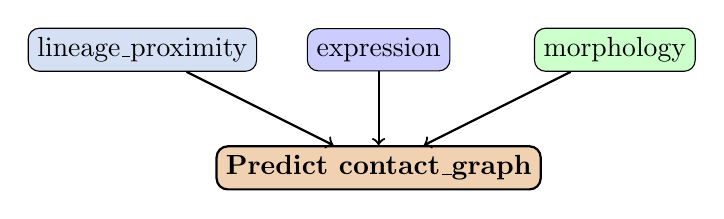
\begin{tikzpicture}
    \node[draw,rounded corners,fill=lineage!20] (prior) at (0,0) {lineage\_proximity};
    \node[draw,rounded corners,fill=blue!20] (expr) at (3,0) {expression};
    \node[draw,rounded corners,fill=green!20] (morph) at (6,0) {morphology};
    
    \node[draw,rounded corners,fill=contact!30,thick] (pred) at (3,-1.5) {\textbf{Predict contact\_graph}};
    
    \draw[->,thick] (prior) -- (pred);
    \draw[->,thick] (expr) -- (pred);
    \draw[->,thick] (morph) -- (pred);
\end{tikzpicture}
\end{center}
\end{frame}

% ============================================================
\section{Scientific Significance}
% ============================================================

\begin{frame}{Why Predict Contact Graphs?}
\begin{block}{1. Cell Fate Depends on Neighbors}
\begin{itemize}
    \item \textbf{Notch signaling}: Requires direct cell-cell contact
    \item \textbf{Induction}: Classic experiments show neighbors influence fate
    \item \textbf{Lateral inhibition}: Adjacent cells adopt different fates
\end{itemize}
\end{block}

\begin{block}{2. Enables Complete Spatial GNN}
\begin{itemize}
    \item Spatial GNN requires neighbor graph
    \item Early cells: Use true \texttt{contact\_graph}
    \item Late cells: Use predicted contacts
    \item $\Rightarrow$ \textbf{Complete spatial modeling} from zygote to adult
\end{itemize}
\end{block}

\begin{block}{3. Scientific Hypothesis}
\textit{Developmental history (ancestor contact) + current state (expression, morphology) can predict current spatial neighbors.}
\end{block}
\end{frame}

\begin{frame}{Link Prediction as Machine Learning Task}
\begin{columns}
\column{0.55\textwidth}
\textbf{Task Formulation}:

\vspace{0.5em}
Given:
\begin{itemize}
    \item Node features: expression + morphology + lineage
    \item Edge prior: \texttt{lineage\_proximity}
    \item Labels: \texttt{contact\_graph} (where available)
\end{itemize}

\vspace{0.5em}
Learn:
\[
P(\text{contact}_{ij} | \text{proximity}_{ij}, \mathbf{x}_i, \mathbf{x}_j)
\]

\vspace{0.5em}
Predict: Contacts for late-stage cells

\column{0.42\textwidth}
\begin{block}{Data Split}
\begin{tabular}{lr}
\toprule
Set & Cells \\
\midrule
Training & 3,790 \\
Prediction & 16,149 \\
No lineage & 214,949 \\
\bottomrule
\end{tabular}
\end{block}

\vspace{0.5em}
\small
Training cells: Have both true contacts AND lineage proximity

Prediction cells: Have lineage proximity but no true contacts
\end{columns}
\end{frame}

\begin{frame}{Broader Impact: Complete Developmental Modeling}
\begin{center}
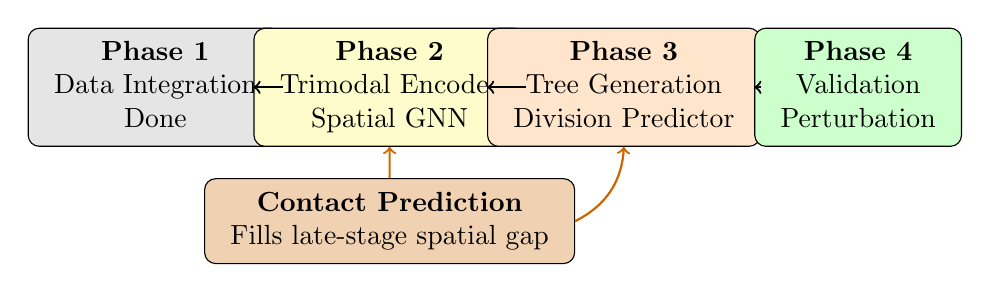
\begin{tikzpicture}[scale=0.85]
    % Pipeline
    \node[draw,rounded corners,fill=gray!20,minimum width=2.5cm] (p1) at (-5,0) {
        \begin{tabular}{c}
        \textbf{Phase 1}\\
        Data Integration\\
        \checkmark Done
        \end{tabular}
    };
    
    \node[draw,rounded corners,fill=yellow!20,minimum width=2.5cm] (p2) at (-1.5,0) {
        \begin{tabular}{c}
        \textbf{Phase 2}\\
        Trimodal Encoder\\
        Spatial GNN
        \end{tabular}
    };
    
    \node[draw,rounded corners,fill=orange!20,minimum width=2.5cm] (p3) at (2,0) {
        \begin{tabular}{c}
        \textbf{Phase 3}\\
        Tree Generation\\
        Division Predictor
        \end{tabular}
    };
    
    \node[draw,rounded corners,fill=green!20,minimum width=2.5cm] (p4) at (5.5,0) {
        \begin{tabular}{c}
        \textbf{Phase 4}\\
        Validation\\
        Perturbation
        \end{tabular}
    };
    
    \draw[->,thick] (p1) -- (p2);
    \draw[->,thick] (p2) -- (p3);
    \draw[->,thick] (p3) -- (p4);
    
    % Contact prediction contribution
    \node[draw,rounded corners,fill=contact!30,minimum width=4cm] (contact) at (-1.5,-2) {
        \begin{tabular}{c}
        \textbf{Contact Prediction}\\
        Fills late-stage spatial gap
        \end{tabular}
    };
    
    \draw[->,thick,contact] (contact) -- (p2);
    \draw[->,thick,contact] (contact.east) to[bend right] (p3.south);
\end{tikzpicture}
\end{center}

\vspace{0.5em}
\textbf{Key Contribution}: Contact prediction enables complete spatial modeling across all developmental stages, not just the CShaper coverage window.
\end{frame}

% ============================================================
\section{Technical Implementation}
% ============================================================

\begin{frame}{Implementation Highlights}
\begin{columns}
\column{0.48\textwidth}
\begin{block}{GPU Acceleration}
\begin{itemize}
    \item PyTorch for expression similarity
    \item 234K $\times$ 231 correlation: 6 seconds
    \item A100 GPU utilized for matrix ops
\end{itemize}
\end{block}

\begin{block}{Optimized Data Structures}
\begin{itemize}
    \item Sparse matrices for graphs
    \item Cached consensus morphology
    \item Vectorized operations
\end{itemize}
\end{block}

\column{0.48\textwidth}
\begin{block}{AnnData Structure}
\footnotesize
\texttt{adata.X} -- Expression\\
\texttt{adata.obsm['X\_spatial']}\\
\texttt{adata.obsm['X\_lineage\_binary']}\\
\texttt{adata.obsp['contact\_binary']}\\
\texttt{adata.obsp['lineage\_proximity']}\\
\texttt{adata.obs['has\_true\_contact']}\\
\texttt{adata.obs['has\_lineage\_proximity']}
\end{block}
\end{columns}

\vspace{0.5em}
\begin{block}{Processing Time}
Full pipeline (234,888 cells): \textbf{$\sim$9 minutes} on A100 GPU
\end{block}
\end{frame}

% ============================================================
\section{Next Steps}
% ============================================================

\begin{frame}{Immediate Next Steps}
\begin{enumerate}
    \item \textbf{Implement Link Prediction Model}
    \begin{itemize}
        \item GNN-based edge predictor
        \item Input: node features + lineage proximity prior
        \item Output: contact probability
    \end{itemize}
    
    \vspace{0.5em}
    \item \textbf{Validate Predictions}
    \begin{itemize}
        \item Cross-validation on early-stage cells
        \item Literature validation (known tissue neighbors)
        \item Connectome consistency (neurons that synapse should be neighbors)
    \end{itemize}
    
    \vspace{0.5em}
    \item \textbf{Integrate with Spatial GNN}
    \begin{itemize}
        \item Use predicted contacts as edges
        \item Aggregate neighbor information for cell state prediction
    \end{itemize}
\end{enumerate}
\end{frame}

\begin{frame}{Long-Term Vision}
\begin{center}
\Large
\textit{``From a single zygote, generate the complete developmental trajectory of an organism --- every cell's state, position, and neighbor relationships, from fertilization to adulthood.''}
\end{center}

\vspace{1em}
\textbf{Contact graph prediction is a critical step toward this vision:}
\begin{itemize}
    \item Bridges the temporal gap in spatial data
    \item Enables complete cell-cell communication modeling
    \item Tests the hypothesis that spatial organization is predictable from developmental history
\end{itemize}

\vspace{1em}
\begin{block}{Key Question}
\textit{Is the spatial organization of \textit{C. elegans} as deterministic as its cell lineage?}
\end{block}
\end{frame}

% ============================================================
% Summary
% ============================================================

\begin{frame}{Summary}
\begin{columns}
\column{0.48\textwidth}
\begin{block}{Completed}
\begin{itemize}
    \item[\checkmark] CShaper data integration
    \item[\checkmark] 40\% morphology coverage
    \item[\checkmark] True contact graph (direct matches)
    \item[\checkmark] Lineage proximity prior
    \item[\checkmark] Training/prediction split
    \item[\checkmark] GPU-accelerated pipeline
\end{itemize}
\end{block}

\column{0.48\textwidth}
\begin{block}{Key Insight}
\begin{itemize}
    \item Ancestor contact $\neq$ descendant contact
    \item But ancestor contact $\rightarrow$ \textbf{prior} for prediction
    \item Link prediction: Learn the mapping
\end{itemize}
\end{block}

\begin{block}{Scientific Contribution}
Testing whether spatial organization follows from developmental history + cell state
\end{block}
\end{columns}
\end{frame}

\begin{frame}
\centering
\Huge Thank You

\vspace{2em}
\Large Questions?
\end{frame}

\end{document}
